\documentclass[11pt]{article}
%Gummi|065|=)
\usepackage[top=1in, bottom=1in, left=0.5in, right=0.5in]{geometry}
\usepackage{graphicx}
\title{Analysis of profiling data: A CS296 Report by Group 28}
\author{Venkata Dinesh (120050051)\\
\texttt {dineshkota3@cse.iitb.ac.in}\and
Nitish Chandra (120050071)\\
\texttt{nitish@cse.iitb.ac.in}\and
Kota Mahindar (120050073)\\
\texttt{mahindar@cse.iitb.ac.in}
}
\date{}
\begin{document}
\maketitle
\section{Analysis of Lab5}
We have run the program for iteration values ranging from 1 to 100. And by observing the plots we have arrived at the following deductions.
\subsection{{\tt time} vs {\tt gettimeofday}}
By analysing the times obtained by {\tt gettimeofday} for various iteration values we observed that it increases when heavy system processes are being run in parallel to it. The time obtained for a function using {\tt gettimeofday} returns the time taken by the function to finish its operation i.e. this time is analogous to the time we calculate using a stopwatch i.e. the time between when the functions is called and when it finishes. It may include the time of other operations which the system may perform by interrupting function's operation.

The {\tt time} command returns three types of times namely real, usr and sys. By analysing these three times for various iteration values, we observed that ``real" time increases when heavy system processes are being run in parallel to it.This is due to the fact that ``real" time returns the time the program takes as a whole to execute i.e. it is analogous to the time which {\tt gettimeofday} returns if it is present at the beginning and end of the program. Unlike ``real" time, ``sys" time returns the time taken by the kernel like allocating memory and such kernel mode services. The ``usr" time is the time taken by the program alone, it does not include the time taken by the kernel.

We have observed that sometimes the sum of ``usr" and ``sys" time is greater and sometimes less than the ``real" time. This is because this relation is dependent on the system, that is if multiple threads run the program then ``sys" and ``usr" time gives the sum of times of threads unlike the real time. Hence we cannot determine any relation between them.

\subsection{Analysis of the Plots}
We have analysed the plots of the data generated for iteration values ranging from 1 to 100 and for 150 reruns each without running any  processes in parallel
to the program

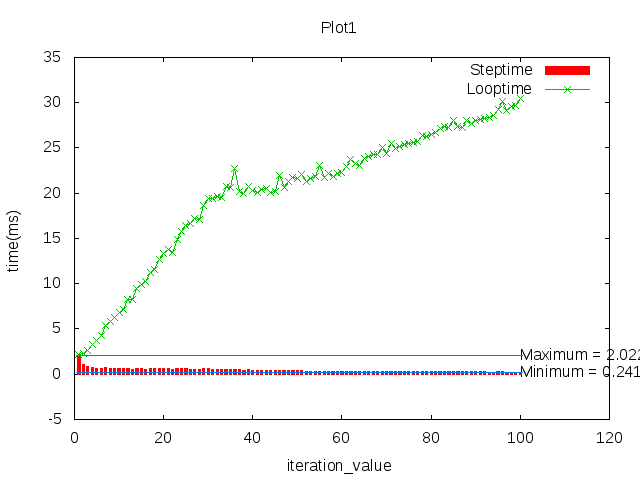
\includegraphics[scale=0.5]{g28_plot01.png}
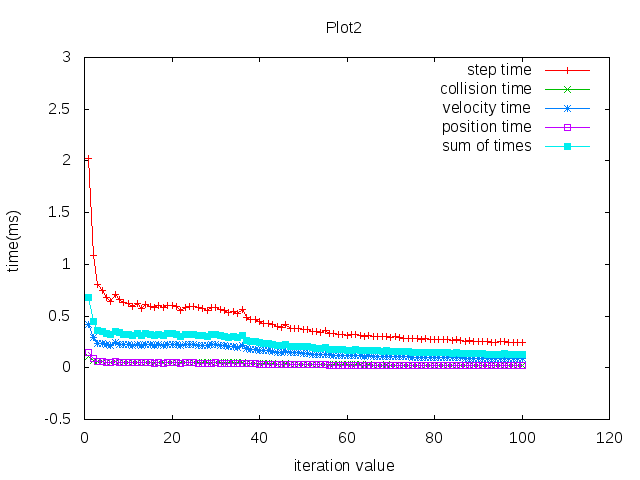
\includegraphics[scale=0.5]{g28_plot02.png}

From Plot1 we can observe that {\bf loop time} increases with increasing iteration value. Since with increase in iteration value, we also increase the number of times the loop runs, it is natural for the {\bf loop time} to increase with the iteration value.

From Plot2 we observe that {\bf collision time, velocity time, position time} decrease with increase in iteration value. This is because collision time is the time taken by program to detect the collision, find the values of collision parameters etc.. To find these values, some subroutines are invoked. When these functions are called, kernel sometimes interrupts the process to allocate time for other processes. So, this interruption time is included in {\bf collision time}.  By observing the data, we can conclude that the increase in total interruption time with iteration number is very less.
$$average collision time = \left(\sum c_i +  total interruption time\right)/v$$ where $v$ is the number of iterations and $c_i$ is the collision time for $i$th iteration. Since the rate of increase of total interruption time  is $<<$ 1, and $c_i$ is nearly same except for the instances when collision happens and these instances occur with a gap of many iteration values, average collision time decreases with increase in iteration value.
 
Similar reason explains the decreasing trend of {\bf velocity time, position time} with respect to iteration value.


We can observe from Plot1 that the average {\bf steptime} is decreasing with increasing iteration number. From Plot2 we can observe that sum of {\bf collision time, position time, velocity time} is strictly less than {\bf step time}, the reason being {\bf step time} includes the time taken to calculate positions, velocities, collision parameters for the next step and also time for which this program is interrupted by kernel. Since all the parameters decrease with increase in iteration value, {\bf step time} also decreases with iteration number.

\centerline{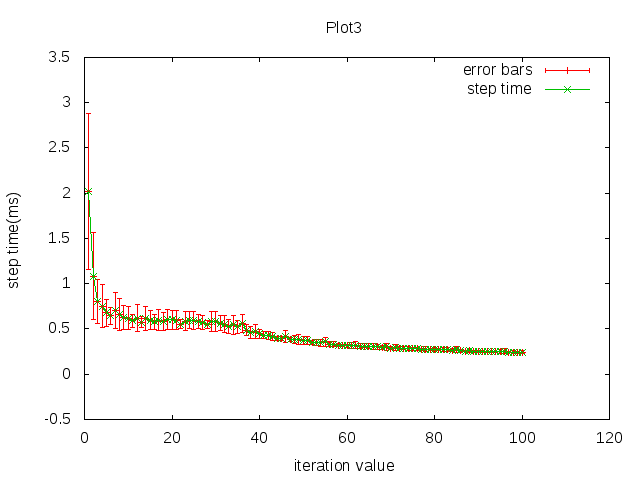
\includegraphics[scale=0.7]{g28_plot03}}

From the above plot, we can observe that,as the {\bf step time} decreases, error in step time also decreases. The error in {\bf step time} arises because, total interruption time usually varies with time. As the iteration value increases, both the average {\bf step time} and average interruption time decrease, so the error associated with {\bf step time}
also decreases.

\centerline{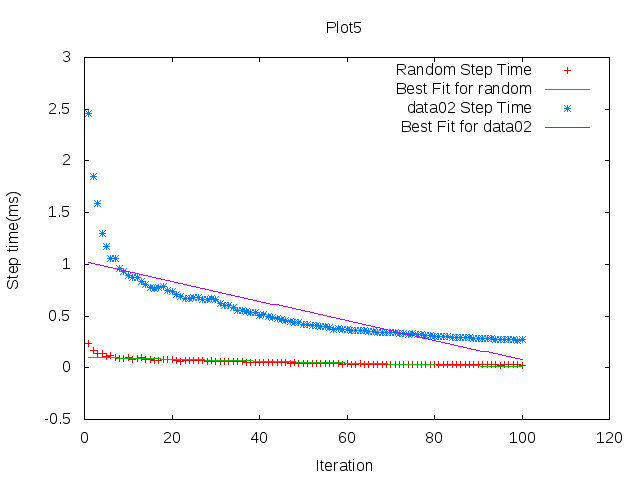
\includegraphics[scale=0.7]{g28_plot05}}
In the above plot, we can see that average {\bf step time} for 150 reruns is always above the average {\bf step time} for random sample of 15 iterations. This suggests that, interruption time contributes less to this random sample. This implies that there is a low probability for an interruption to occur. From the graph, we can assert that although there is a low probability for an interruption to occur, value of interruption time is considerable when compared to original {\bf step time}.
\section{Profiling}
We have chosen {\tt gprof} to profile the code. While increasing the iteration value, for smaller values the profiling times of most of the functions turns out to be zero but on increasing the iteration value they gradually increase since only after a certain iteratons collisons between the objects happen and hence new functions are called.

Hence we have compared the profiling data among larger iterations and by observing the similarities in data in that range we have selected the iteration number as 100000 to generate the interesting profile.
\subsection{Comparison of  Profiles}
The very first difference we observe between the two profiles is that some functions which are present in the ``debug'' flat profile are absent in ``release'' profile. This is because, as {\tt man} page of {\tt gcc} explains, some of the functions for which the result is a constant or the result is already known will not be called when compiled with {\tt -O3} option. Hence, the default constructors like {\tt b2Vec2::b2Vec2()} are present only in ``debug'' profile since they return the same value everytime.


We can also see that {\tt -O3} that we have specified reduces the ``cumulative seconds'' taken by the executable file.The executable file generated using the optimisation options takes only 2.32 seconds whereas the executable  without {\tt -O3} flag takes 11.25 seconds. So, we can conclude that the code indeed gets optimised. 

\subsection{Possible Optimisations}
All the functions of class {\tt b2World} consume less ``self seconds'' when compiled with {\tt -O3} flags when compared to the executable generated without optimisation flags. This indicates that code in class {\tt b2World} can be optimised. 

Number of calls to functions of class {\tt debug\_draw\_t} increase linearly with the iteration number. This implies that for every iteration, the entire screen is redrawn. Hence we can optimise this function by drawing only those bodies which are not static.

Some of the functions in class {\tt b2ContactSolver} like {\tt WarmStart(), SolveVelocityConstraints()} take less time when the {\tt -O3} flag is used and some other functions like {\tt SolvePositionConstrains(), StoreImpulses()} take more time with optimisation. This may be because optimising some of the functions increases the time taken for execution of other functions.

There is a large time gap for methods in classes {\tt b2StackAllocator, b2Timer} with and without the optimisation flags.Hence we can optimise these methods.

\subsection{Call Graphs}

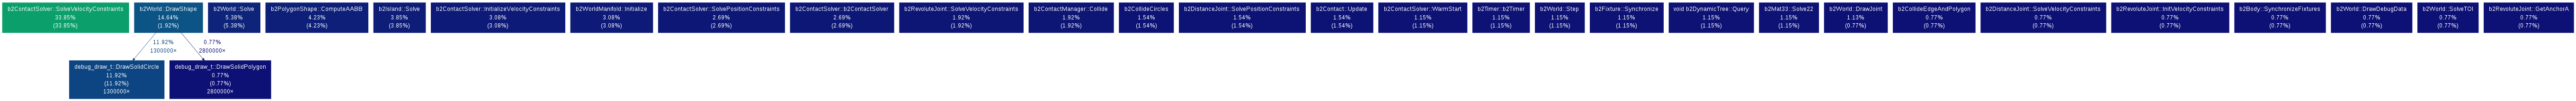
\includegraphics[width=8in,height=2in]{./release.png}

\centerline{\bf release.png}



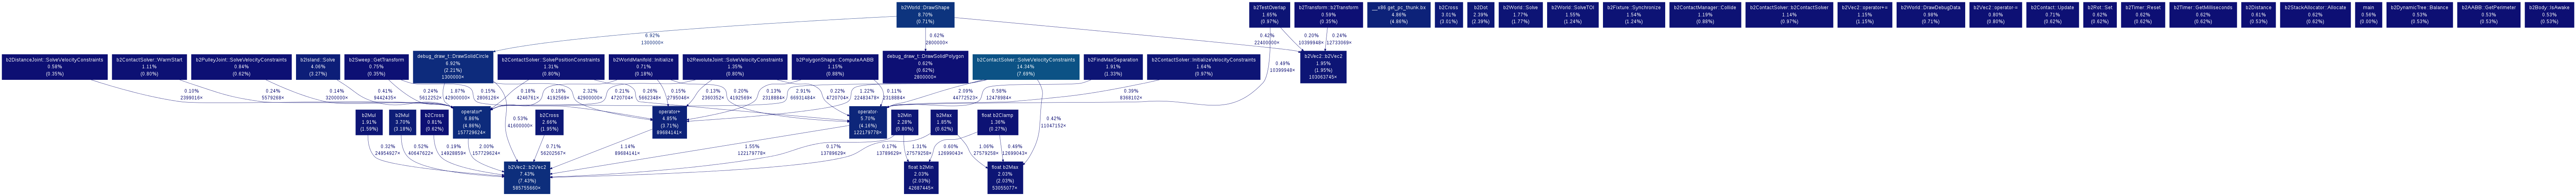
\includegraphics[width=7.7in,height=2in]{./debug.png}

\centerline{\bf debug.png}

In both cases, {\tt b2ContactSolver::SolveVelocityConstraints()} takes the highest percentage of time consumed. From the above two plots, we can see that either many functions have not been invoked or the self time those functions is negligible, when the executable file is generated using {\tt -O3} flag. So, we can infer that all these calls to the functions can be optimised. 
%\centerline{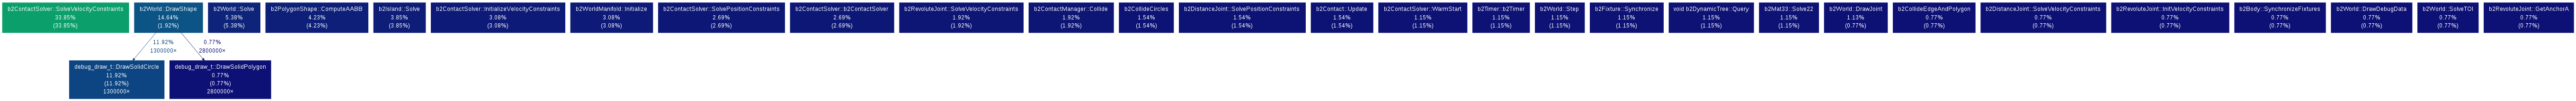
\includegraphics[scale=0.3]{release.png}}

\end{document}